% Festlegung des Allgemeinen Dokumentenformats
\documentclass[a4paper,11pt,headsepline, fleqn, english]{scrartcl}%article

% Umlaute unter UTF8 nutzen
\usepackage[utf8]{inputenc}

% Variablen
%\input{latex_einstellungen/variablen}

% weitere Pakete
% Grafiken aus PNG Dateien einbinden
\usepackage{graphicx}

% Deutsche Sonderzeichen und Silbentrennung nutzen
%\usepackage[ngerman]{babel}

% Eurozeichen einbinden
\usepackage[right]{eurosym}

% Zeichenencoding
\usepackage[T1]{fontenc}

\usepackage{lmodern}

\usepackage{algpseudocode}
\usepackage{algorithm}
\let\oldReturn\Return
\renewcommand{\Return}{\State\oldReturn}

\usepackage{float}
% floatende Bilder ermöglichen
%\usepackage{floatflt}
\usepackage[font=footnotesize]{caption}
%\usepackage{caption}
\usepackage{subcaption}

% mehrseitige Tabellen ermöglichen
\usepackage{longtable}

% Unterstützung für Schriftarten
%\newcommand{\changefont}[3]{ 
	%\fontfamily{#1} \fontseries{#2} \fontshape{#3} \selectfont}

% Packet für Seitenrandabständex und Einstellung für Seitenränder
\usepackage{geometry}
\geometry{left=3.5cm, right=2cm, top=2.5cm, bottom=2.5cm}

% Paket für Boxen im Text
\usepackage{fancybox}

% bricht lange URLs "schön" um
\usepackage[hyphens,obeyspaces,spaces]{url}

% Paket für Textfarben
\usepackage{color}

\usepackage{hyperref}
\hypersetup{
	colorlinks,
	citecolor=black,
	filecolor=black,
	linkcolor=black,
	urlcolor=black
}

% Mathematische Symbole importieren
\usepackage{amssymb}
\usepackage{amsmath}
% auf jeder Seite eine Überschrift (alt, zentriert)
%\pagestyle{headings}

% erzeugt Inhaltsverzeichnis mit Querverweisen zu den Abschnitten (PDF Version)
%\usepackage[bookmarksnumbered,pdftitle={\titleDocument},hyperfootnotes=false]{hyperref}
%\hypersetup{colorlinks, citecolor=red, linkcolor=blue, urlcolor=black}
%\hypersetup{colorlinks, citecolor=black, linkcolor= black, urlcolor=black}

% neue Kopfzeilen mit fancypaket
\usepackage{fancyhdr} %Paket laden
\pagestyle{fancy} %eigener Seitenstil
\fancyhf{} %alle Kopf- und Fußzeilenfelder bereinigen
\fancyhead[L]{\nouppercase{\leftmark}} %Kopfzeile links
\fancyhead[C]{} %zentrierte Kopfzeile
%\fancyhead[R]{Leonie Boland} %Kopfzeile rechts
\renewcommand{\headrulewidth}{0.4pt} %obere Trennlinie
\fancyfoot[C]{\thepage} %Seitennummer
%\renewcommand{\footrulewidth}{0.4pt} %untere Trennlinie

%authoryear-comp
\RequirePackage[style = numeric, backend = biber]{biblatex}
\addbibresource{Bib.bib}

% Paket für Zeilenabstand
\usepackage{setspace}

%new added packages:
\usepackage{listings}
\usepackage{xcolor}
\usepackage[inline]{enumitem}

% use these constant for defining image widths
\newcommand{\oneImgWidth}{\linewidth}
\newcommand{\twoImgWidth}{0.494\linewidth}
\newcommand{\threeImgWidth}{0.326\linewidth}
\newcommand{\fourImgWidth}{0.246\linewidth}
\newcommand{\sixImgWidth}{0.162\linewidth}
\newcommand{\eightImgWidth}{0.120\linewidth}
\newcommand{\nineImgWidth}{0.107\linewidth}

\newcommand{\captionadjust}{\vspace{-8pt}}


\definecolor{codegreen}{rgb}{0,0.6,0}
\definecolor{codegray}{rgb}{0.5,0.5,0.5}
\definecolor{codepurple}{rgb}{0.58,0,0.82}
\definecolor{backcolour}{rgb}{0.95,0.95,0.92}

\lstdefinestyle{mystyle}{
  backgroundcolor=\color{backcolour},   
  commentstyle=\color{codegreen},
  keywordstyle=\color{magenta},
  numberstyle=\tiny\color{codegray},
  stringstyle=\color{codepurple},
  basicstyle=\ttfamily\fontsize{8}{8}\selectfont,
  breakatwhitespace=false,         
  breaklines=true,                 
  captionpos=b,                    
  keepspaces=true,                 
  numbers=left,                    
  numbersep=5pt,                  
  showspaces=false,                
  showstringspaces=false,
  showtabs=false,                  
  tabsize=2
}

\lstset{style=mystyle}

\begin{document}
	\thispagestyle{empty}

\begin{verbatim}
	
	
	
\end{verbatim}

\begin{center}
	\Large{\textbf{Heidelberg University}}
\end{center}


\begin{center}
	\Large{\textbf{End of the Semester Project}}\\
	\Large{Lecture: Machine Learning Essentials}
\end{center}

\begin{verbatim}
	
	
	
\end{verbatim}

\begin{center}
	\large{\textbf{Report}}\\
	\huge{Using Reinforcement Learning Methods to Train an Agent to Play Bomberman}	
\end{center}

\begin{verbatim}
	
	
	
	
	
	
	
	
	
	
	
	
	
	
	
	
\end{verbatim}

% Links unten die wichtigen Daten
\begin{flushleft}
	\begin{tabular}{llll}
		\textbf{Institute:} && Computer Vision and Learning Lab & \\
		&& Biomedical Genomics Group& \\
		&& \\
		\textbf{Authors:} & & Leonie Boland, MatNr. 4055040& \\
		& & Kevin Klein, MatNr. 4114347& \\
		& & Berkay Günes, MatNr. 3446492& \\
		& &\\
		\textbf{Version from:} & & \today &\\
		& & \\
		\textbf{Supervisor:} & & Prof. Dr. Ullrich Köthe &\\
	\end{tabular}
\end{flushleft}
	
	% römische Numerierung
	\pagenumbering{roman}
	
	
	\newpage
	
	% Seitenzählung bei Inhaltsverzeichnis beginnen
	\setcounter{page}{1}
	
	% Inhaltsverzeichnis anzeigen
	\thispagestyle{empty}
	\tableofcontents
	
	\newpage
	
	% arabische Seitennummerierung ab hier
	\pagenumbering{arabic}
	
	\section{Introduction}

	
\fancyhead[R]{Berkay Günes}
%- problem\\
%- brief overview of methods:\\
%- Deep Q Learning give examples where its used (e.g. Mario)\\
%- definitely all methods mentioned in the lecture\\
%- maybe research more possibilities and examples when its used

Building games with artificial agents that learn how to play is a long-standing goal in Game-AI. In this work we focus on building an agent that learns to master the classical arcade game Bomberman with the help of reinforcment learning.\\ \\
In the game Bomberman each agents finds itself in a grid of crates and walls and tries to win the game by collecting as many points as possible in each round.\\
He can achieve this by planting bombs to destroy crates and collect coins or kill other agents. \\
In a game like this, with a lot of options and strategies, it gets rather complicated to play the game and is therefore ideally suited to try solving the game by machine learning.\\ \\
The reinforcement learning (RL) approach, used in this project, is ideally suited for teaching games to AIs as it gives the creator the opportunity to guide the agent into the desired direction by creating rewards and punishments for certain behaviours.\\ \\
In this project we mainly focused on the Q-learning algorithm which learns the value of an action in a particular state and has been proven successful in endeavours like this many times. \\
We further extended our model to a Deep Q-Network, which contains a Neural network to process the feature state of the agent. This gives the benefit of faster computation in an environment with a large feature state, as the classical Q-tables scales exponentially to the given input.\\ \\
The code to our agents can be found on Github: \\
\url{https://github.com/bGuenes/bomberman_MLE_homework} \\ \\
Our model handed in to the tournament is called "agent the destroyer of worlds 2" and is a Neural Network with three convolutions and one linear input layer in parallel, followed by four parallel linear inputs, which then merge together into one fully connected layer and then go to the output layer. The structure of the Network is explained in more detail in section \ref{NetworkS}. \\
The agent "destroyer of students" is based on the same network structure, but with a vision field of 9x9 instead of 7x7.\\
In test before the deadline the agent with the smaller vision field performed best and was therefore handed in.\\
The remaining agents in the repository are predecessors with a simpler Network structure containing just one hidden linear layer.

\newpage
\fancyhead[R]{Leonie Boland}
\subsection{Related Work}

In recent years Deep Q-Learning gained popularity in the field of reinforcement learning for applications in various domains, like video games, robotics and decision making processes. The foundation for Deep Q-Learning was established in the paper 'Playing Atari with Deep Reinforcement Learning' \cite{deepRL}. The authors developed the first successful variant of Q-learning in combination with a convolutional neural network and tested it on seven Atari 2600 games from the Arcade Learning Environment.

Thenceforth the algorithm was further developed in the claim to surpassing human performance in more and more games. Van Hasselt et al. \cite{doubleQ} propose an improvement to Deep Q-learning, called Double Q-learning, due to some weaknesses of the Deep Q-learning algorithm, like overestimating action values. This method was used successfully to train a Mario playing agent using Pytorch \cite{mario}.

Another reinforcement learning technique is Proximal Policy Optimization (PPO) \cite{ppo}. PPO algorithms use trust region constrains and clipped objective functions, that allows multiple epochs of minibatch updates. Advantages of this reinforcement learning method are its stability and sample efficiency, which lead to outmatching other online policy gradient methods in simulated robotic locomotion and Atari games. PPO has been applied on Bomberman in two different variations by Goulart et al. \cite{ppobomberman}. This work compared two Bomberman's agent performances after training one with an imitation-based learner improving with actor-critic PPO and the other only using PPO including either a Multi-Layer Perceptron or a Long Short Term-Memory network. Their conclusion is, that the imitation-based agent operates best. 
	
	\newpage
	\section{Fundamentals}
	
	\fancyhead[R]{Berkay Günes}

In this section, we provide a brief overview of the fundamental machine learning concepts that we 
have applied in both projects. Here, we outline the key principles and techniques that form the foundation 
of our machine learning implementations. These concepts serve as the building blocks for the approaches adopted in both projects

\subsection{Q-Learning}

Reinforcement learning is a subfield of machine learning that focuses on training agents to make a decision given a state representation of the world through trial and error, aiming to maximize a cumulative reward. Q-learning is a fundamental RL algorithm that has played a pivotal role in solving various problems in robotics, gaming, and more. In this section, we will introduce Q-learning and then focus on Deep Q-Networks (DQNs), explaining how they differ from traditional Q-tables.

\subsubsection{Q-Learning}

Q-learning is a model-free RL algorithm that learns an action-value function, denoted as \(Q(s, a)\), where 's' represents the state, and 'a' represents the action. The Q-value of a state-action pair quantifies the expected cumulative reward an agent can achieve starting from that state and taking a specific action. The primary goal of Q-learning is to find the optimal policy, which is a mapping of states to actions that maximizes the expected cumulative reward over time.

The Q-learning algorithm updates Q-values iteratively through the following equation:

\begin{equation}
	Q(s_t, a_t) \leftarrow Q(s_t, a_t) + \alpha \left[ r_t + \gamma \max_a Q(s_{t+1}, a) - Q(s_t, a_t) \right]
\end{equation}

Here, \(s_t\) represents the current state, \(a_t\) is the chosen action, \(r_t\) is the immediate reward received, \(\gamma\) is the discount factor, and \(\alpha\) is the learning rate.

Q-learning operates in discrete state and action spaces, making it highly suitable for problems where these spaces are well-defined, such as board games and simple robotic tasks. However, Q-learning faces limitations when dealing big feature spaces as the Q-tables grow exponentially, which led to the development of Deep Q-Networks (DQNs).

\subsubsection{Deep Q-Networks}

Deep Q-Networks are a class of neural network-based RL algorithms that combine deep learning with Q-learning principles. They address the limitations of Q-learning by approximating the Q-value function using a neural network instead of a Q-table. This enables DQNs to handle complex and continuous state spaces, making them highly effective in tasks like image-based game playing and autonomous driving.

Key differences between DQNs and traditional Q-tables include:

\begin{enumerate}
	\item \textbf{Function Approximation}: DQNs use a neural network to approximate the Q-values, allowing them to generalize across similar states. Traditional Q-learning relies on a discrete Q-table, which is not practical for large state spaces.
	
	\item \textbf{Experience Replay}: DQNs store experiences (state, action, reward, next state) in a replay buffer and sample mini-batches during training. This stabilizes learning by breaking the temporal correlation between experiences and mitigating the risk of convergence to suboptimal policies.
	
	\item \textbf{Target Network}: To stabilize training, DQNs use two networks: the target network and the policy network. The target network lags behind the policy network, and its Q-values are used as targets for training. This helps in reducing the variance of Q-value estimates during training.
\end{enumerate}

% ----------------------------------------------------------------------------------------------------------------------------------------------

\subsection{Neural Networks}
Neural networks, often referred to as artificial neural networks (ANNs), are a class of machine learning models inspired by the structure and function of the human brain. They have gained significant popularity in recent years due to their remarkable ability to learn and generalize from data, making them versatile tools for a wide range of tasks, from image recognition to natural language processing. While they have been around for a rather long time, it was only in the recent decade that computational power became sufficient to train networks that are large enough to be useful. Also, the amount of available data for training has dramatically increased over the years.

\subsubsection{Basic Structure of a Neural Network}

At its core, a neural network is composed of interconnected nodes, known as neurons or artificial neurons, organized into layers. The three primary types of layers in a neural network are:

\begin{enumerate}
	\item \textbf{Input Layer}: This layer consists of neurons that receive the initial data or features. Each neuron corresponds to a specific feature, and its value represents the magnitude of that feature.
	
	\item \textbf{Hidden Layers}: Hidden layers are intermediary layers between the input and output layers. They process the input data through a series of weighted connections and nonlinear activation functions.
	
	\item \textbf{Output Layer}: The output layer produces the final results or predictions of the neural network's task. The number of neurons in this layer depends on the problem, with each neuron typically corresponding to a different class or a particular aspect of the prediction.
\end{enumerate}

\subsubsection{Working Principle of Neurons}

Each neuron in a neural network performs a simple but crucial task. It takes in a weighted sum of its inputs, adds a bias term, and passes this value through an activation function to produce an output, thus each neuron in the network has a number of free parameters that need to be determined by training. The equation for the operation of a neuron is be defined as:
\begin{equation}
	\text{Output} = \text{Activation}\left(\sum_{i=1}^{n} (\text{Input}_i \times \text{Weight}_i) + \text{Bias}\right)
\end{equation}

\subsubsection{Training a Neural Network}

The essence of neural networks lies in their ability to approximate any function, and thus "learn" a relation between input and output data, no matter how complex this relationship might be. This learning process involves adjusting the weights and biases of the neurons to minimize a specific loss or error function. Here's an overview of the training process:

\begin{enumerate}
	\item \textbf{Forward Pass}: During the forward pass, input data is propagated through the network layer by layer. Neurons compute their outputs using the weighted sum and activation function.
	
	\item \textbf{Loss Calculation}: The output of the neural network is compared to the ground truth or target values, and a loss (error) is calculated. The choice of loss function depends on the task. A few different examples are given in \ref{loss}.
	
	\item \textbf{Backpropagation}: In the backpropagation step, the gradient of the loss with respect to the network's parameters (weights and biases) is computed using the chain rule. This gradient indicates how much each parameter should be adjusted to minimize the loss.
	
	\item \textbf{Optimization}: The gradients are used to update the network's parameters in the opposite direction of the gradient. This process is repeated iteratively until the loss converges to a minimum.
\end{enumerate}

\subsubsection{Batch Normalization}

Batch Normalization is a widely used technique in deep learning, specifically designed to address training instability and accelerate convergence in neural networks. It operates by normalizing the activations of each layer within mini-batches during training and introduce learnable parameters (scale and shift) to allow the network to adapt and fine-tune the normalized activations.
These are then passed through the activation function and used in subsequent layers for forward and backward passes.
\\ \\
\textbf{Advantages of Batch Normalization:} \\
Batch Normalization helps mitigate issues like vanishing and exploding gradients, making it easier to train deep networks. By normalizing the activations, it maintains a more consistent and stable gradient flow during backpropagation.
Neural networks with Batch Normalization also tend to converge faster. The normalization of activations helps prevent the network from getting stuck in plateaus, enabling quicker convergence to a better solution.
Batch Normalization introduces a degree of regularization by reducing internal covariate shift (the change in the distribution of activations between layers). This often leads to better generalization and reduced overfitting.

%------------------------------------------------------------------------------------------------------------------------------

\subsection{Loss Functions} \label{loss}

Loss functions play a crucial role in training neural networks. They quantify the difference between the predicted outputs of the model and the ground truth labels. Different loss functions are used for different types of tasks and data.

\subsubsection{Cross-Entropy Loss} \label{sec:crossentropy}

Cross-entropy loss, often used in classification tasks, measures the dissimilarity between predicted class probabilities and the true class labels. It is particularly suitable for problems where the outputs are probability distributions.

The equation for binary cross-entropy loss for a single example is:
\begin{align}
	\text{Binary Cross-Entropy Loss} = -\left(y \log(\hat{y}) + (1 - y) \log(1 - \hat{y})\right)
\end{align}

Preferred Use Case: Cross-entropy loss is commonly used in classification tasks, including image classification and natural language processing.

\subsubsection{Huber Loss}

Huber loss is a robust loss function that combines the best properties of Mean Absolute Error (MAE) and Mean Squared Error (MSE) loss functions. It is less sensitive to outliers and provides a smoother gradient compared to MSE.

The Huber loss is defined as:
\begin{align}
	\text{Huber Loss} = \begin{cases}
		\frac{1}{2}(\hat{y} - y)^2, & \text{if } |\hat{y} - y| \leq \delta \\
		\delta|\hat{y} - y| - \frac{1}{2}\delta^2, & \text{otherwise}
	\end{cases}
\end{align}

Preferred Use Case: Huber loss is useful when dealing with regression problems where the dataset may contain outliers.

\subsubsection{Mean Squared Error (MSE) Loss}

Mean Squared Error (MSE) loss is a common loss function used for regression tasks. It measures the average squared difference between predicted and true values.

The equation for MSE loss is:
\begin{align}
	\text{MSE Loss} = \frac{1}{n} \sum_{i=1}^{n} (\hat{y}_i - y_i)^2    
\end{align}

Preferred Use Case: MSE loss is suitable for regression problems where the goal is to minimize the squared difference between predicted and true values.

\subsubsection{Smooth L1 Loss}

Smooth L1 loss is another loss function for regression that combines the best of both MAE and MSE. It is less sensitive to outliers than MSE and provides a smooth gradient.

The equation for Smooth L1 loss is:
\begin{align}
	\text{Smooth L1 Loss} = \begin{cases}
		0.5(\hat{y} - y)^2, & \text{if } |x| < 1 \\
		|x| - 0.5, & \text{otherwise}
	\end{cases}    
\end{align}

Preferred Use Case: Smooth L1 loss is suitable for regression problems, especially when dealing with data that may contain outliers.

\subsubsection{Optimal Loss Function for Bomberman}

Selecting the most suitable loss function for reinforcement learning in the context of playing the arcade game Bomberman requires careful consideration of the game's dynamics and objectives.\\
Cross-entropy loss is typically used for classification tasks and may not be the most appropriate choice for Bomberman. It focuses on estimating class probabilities, which may not align well with the continuous and dynamic nature of the game. \\
The Huber loss is designed to be robust to outliers, which could be beneficial in Bomberman, as the agent may encounter unexpected scenarios and rewards. However, it is primarily used for regression tasks, and its effectiveness in RL settings might vary. \\
MSE loss measures the squared difference between predicted and target values. In the context of Bomberman, where the agent's goal is to maximize cumulative rewards, using MSE loss could lead to convergence issues. It tends to focus on minimizing deviations from the target, which might not be the primary objective in a dynamic game like Bomberman. \\
Smooth L1 loss combines the benefits of both Huber and MSE losses. It provides a smooth gradient and is less sensitive to outliers. For Bomberman, where the agent needs to balance exploration and exploitation, Smooth L1 loss could be a reasonable choice, as it encourages stable learning without being overly sensitive to small fluctuations in rewards.

% ----------------------------------------------------------------------------------------------------------------------------------------------
\subsection{Optimizer}

In machine learning, optimization plays a vital role in training deep neural networks. Optimizers are algorithms responsible for adjusting the model's parameters to minimize a loss function during training. They control how the model learns and, consequently, impact its convergence speed and overall performance. Two popular optimizers used in deep learning are RMSprop and AdamW. In this section, we will explain the role of optimizers and delve into the mechanisms of RMSprop and AdamW.

Optimizers in machine learning are responsible for updating the weights and biases of a neural network to minimize a chosen loss function. The primary goal is to find the optimal set of parameters that result in the lowest possible loss. This is achieved through an iterative process that involves computing gradients of the loss with respect to the model's parameters and adjusting these parameters in the direction that reduces the loss.

\subsubsection{RMSprop}

RMSprop (Root Mean Square Propagation) is an adaptive learning rate optimizer designed to address the issue of slow convergence in stochastic gradient descent (SGD) and is defined by:


\begin{align}
	v_t &= \beta \cdot v_{t-1} + (1 - \beta) \cdot (\nabla J(\theta_t))^2 
	\\
	\theta_{t+1} &= \theta_t - \frac{\alpha}{\sqrt{v_t + \epsilon}} \cdot \nabla J(\theta_t)
\end{align}    

Where \(v_t\) describes the moving average of squared gradients, \(\beta\) the decay rate for the moving average (usually set to a value like 0.9), \(\nabla J(\theta_t)\) represents the gradient of the loss with respect to the model parameters \(\theta_t\), \(\alpha\) is the learning rate and\(\epsilon\) is a small constant (typically used to avoid division by zero).

RMSprop works by maintaing a moving average of squared gradients for each parameter. It then adapts the learning rates individually for each parameter by dividing the current gradient by the square root of the moving average of squared gradients.
This adaptation helps to scale down the learning rate for parameters with high variance in gradients and scale up the learning rate for those with low variance.
RMSprop includes a smoothing term to avoid dividing by very small values, ensuring stable convergence.

RMSprop is well-suited for tasks with non-stationary objectives or sparse data. It helps mitigate the vanishing and exploding gradient problems and often converges faster than traditional SGD.

\subsubsection{AdamW}

AdamW (Adam with Weight Decay) is a variant of the Adam optimizer that addresses weight decay issues. AdamW incorporates L2 regularization (weight decay) directly into the parameter update step, unlike the original Adam optimizer, which applies weight decay as an additional term after the parameter update. It is defined by:

\begin{align}
	m_t &= \beta_1 \cdot m_{t-1} + (1 - \beta_1) \cdot \nabla J(\theta_t) \\
	v_t &= \beta_2 \cdot v_{t-1} + (1 - \beta_2) \cdot (\nabla J(\theta_t))^2 \\
	\hat{m}_t &= \frac{m_t}{1 - \beta_1^t} \\
	\hat{v}_t &= \frac{v_t}{1 - \beta_2^t} \\
	\theta_{t+1} &= \theta_t - \frac{\alpha}{\sqrt{\hat{v}_t + \epsilon}} \cdot \hat{m}_t - \lambda \cdot \theta_t
\end{align}

Where \(m_t\) and \(v_t\) are the first and second moments of gradients, respectively, \(\beta_1\) and \(\beta_2\) are the exponential decay rates for the first and second moments (typically set to values like 0.9 and 0.999), \(\hat{m}_t\) and \(\hat{v}_t\) are bias-corrected estimates of the moments, \(\nabla J(\theta_t)\) represents the gradient of the loss with respect to the model parameters \(\theta_t\), \(\alpha\) is the learning rate, \(\epsilon\) is a small constant and \(\lambda\) is the weight decay term, which adds L2 regularization to the parameter updates. \\
AdamW computes the gradients of the loss and updates the moving averages of the first and second moments of gradients.
It then includes an L2 regularization term in the parameter update step, which helps prevent overfitting.
By integrating weight decay, AdamW offers better generalization and improved performance in tasks with large neural networks.\\

AdamW is generally well-suited for a wide range of deep learning tasks and is particularly effective when dealing with large networks and complex datasets.

\subsubsection{Choosing the Right Optimizer}

The choice between RMSprop and AdamW depends on the specific characteristics of the deep learning task:

\begin{itemize}
	\item \textbf{RMSprop}: When dealing with non-stationary objectives, sparse data, or tasks where adaptive learning rates are crucial. It can help in scenarios where the learning rate needs to vary across parameters.
	
	\item \textbf{AdamW}: When you require effective regularization through weight decay, especially in large neural networks with many parameters. It is suitable for tasks where preventing overfitting is a top priority.
\end{itemize}

In practice, experimenting with both optimizers on the specific dataset and model architecture is often the best way to determine which one performs better for the task.

% ----------------------------------------------------------------------------------------------------------------------------------------------



	
	\newpage
	\section{Methods}
	
	\fancyhead[R]{Berkay Günes}

In this section, we elucidate our methodology and approaches concerning the various machine learning models 
that we have developed for the Bomberman game agent. We will also substantiate what has proven effective, articulate 
the concepts we have discarded, and expound upon the rationale for ultimately selecting the model we have submitted.

\subsection{Q-learning}

Reinforcement learning (RL) is a subfield of machine learning that focuses on training agents to make a decision given a state representation of the world through trial and error, aiming to maximize a cumulative reward. Q-learning is a fundamental RL algorithm that has played a pivotal role in solving various problems in robotics, gaming, and more. In this section, we will introduce Q-learning and then focus on Deep Q-Networks (DQNs), explaining how they differ from traditional Q-tables.

\subsubsection{Q-Learning}

Q-learning is a model-free reinforcement learning algorithm that learns an action-value function, denoted as \(Q(s, a)\), where 's' represents the state, and 'a' represents the action. The Q-value of a state-action pair quantifies the expected cumulative reward an agent can achieve starting from that state and taking a specific action. The primary goal of Q-learning is to find the optimal policy, which is a mapping of states to actions that maximizes the expected cumulative reward over time.

The Q-learning algorithm updates Q-values iteratively through the following equation:

\begin{equation}
	Q(s_t, a_t) \leftarrow Q(s_t, a_t) + \alpha \left[ r_t + \gamma \max_a Q(s_{t+1}, a) - Q(s_t, a_t) \right]
\end{equation}

Here, \(s_t\) represents the current state, \(a_t\) is the chosen action, \(r_t\) is the immediate reward received, \(\gamma\) is the discount factor, and \(\alpha\) is the learning rate.

Q-learning operates in discrete state and action spaces, making it highly suitable for problems where these spaces are well-defined, such as board games and simple robotic tasks. However, Q-learning faces limitations when dealing big feature spaces as the Q-tables grow exponentially, which led to the development of Deep Q-Networks (DQNs).

\subsubsection{Deep Q-Networks}

Deep Q-Networks (DQNs) are a class of neural network-based reinforcement learning algorithms that combine deep learning with Q-learning principles. They address the limitations of Q-learning by approximating the Q-value function using a neural network instead of a Q-table. This enables DQNs to handle complex and continuous state spaces, making them highly effective in tasks like image-based game playing and autonomous driving.

Key differences between DQNs and traditional Q-tables include:

\begin{enumerate}
	\item \textbf{Function Approximation}: DQNs use a neural network to approximate the Q-values, allowing them to generalize across similar states. Traditional Q-learning relies on a discrete Q-table, which is not practical for large state spaces.
	
	\item \textbf{Experience Replay}: DQNs store experiences (state, action, reward, next state) in a replay buffer and sample mini-batches during training. This stabilizes learning by breaking the temporal correlation between experiences and mitigating the risk of convergence to suboptimal policies.
	
	\item \textbf{Target Network}: To stabilize training, DQNs use two networks: the target network and the policy network. The target network lags behind the policy network, and its Q-values are used as targets for training. This helps in reducing the variance of Q-value estimates during training.
\end{enumerate}

% ----------------------------------------------------------------------------------------------------------------------------------------------

\subsection{Neural Networks}
Neural networks, often referred to as artificial neural networks (ANNs), are a class of machine learning models inspired by the structure and function of the human brain. They have gained significant popularity in recent years due to their remarkable ability to learn and generalize from data, making them versatile tools for a wide range of tasks, from image recognition to natural language processing. While they have been around for a rather long time, it was only in the recent decade that computational power became sufficient to train networks that are large enough to be useful. Also, the amount of available data for training has dramatically increased over the years.

\subsubsection{Basic Structure of a Neural Network}

At its core, a neural network is composed of interconnected nodes, known as neurons or artificial neurons, organized into layers. The three primary types of layers in a neural network are:

\begin{enumerate}
	\item \textbf{Input Layer}: This layer consists of neurons that receive the initial data or features. Each neuron corresponds to a specific feature, and its value represents the magnitude of that feature.
	
	\item \textbf{Hidden Layers}: Hidden layers are intermediary layers between the input and output layers. They process the input data through a series of weighted connections and nonlinear activation functions.
	
	\item \textbf{Output Layer}: The output layer produces the final results or predictions of the neural network's task. The number of neurons in this layer depends on the problem, with each neuron typically corresponding to a different class or a particular aspect of the prediction.
\end{enumerate}

\subsubsection{Working Principle of Neurons}

Each neuron in a neural network performs a simple but crucial task. It takes in a weighted sum of its inputs, adds a bias term, and passes this value through an activation function to produce an output, thus each neuron in the network has a number of free parameters that need to be determined by training. The equation for the operation of a neuron is be defined as:

\begin{equation}
	\text{Output} = \text{Activation}\left(\sum_{i=1}^{n} (\text{Input}_i \times \text{Weight}_i) + \text{Bias}\right)
\end{equation}

\subsubsection{Training a Neural Network}

The essence of neural networks lies in their ability to approximate any function, and thus "learn" a relation between input and output data, no matter how complex this relationship might be. This learning process involves adjusting the weights and biases of the neurons to minimize a specific loss or error function. Here's an overview of the training process:

\begin{enumerate}
	\item \textbf{Forward Pass}: During the forward pass, input data is propagated through the network layer by layer. Neurons compute their outputs using the weighted sum and activation function.
	
	\item \textbf{Loss Calculation}: The output of the neural network is compared to the ground truth or target values, and a loss (error) is calculated. The choice of loss function depends on the task. A few different examples are given in \ref{loss}.
	
	\item \textbf{Backpropagation}: In the backpropagation step, the gradient of the loss with respect to the network's parameters (weights and biases) is computed using the chain rule. This gradient indicates how much each parameter should be adjusted to minimize the loss.
	
	\item \textbf{Optimization}: The gradients are used to update the network's parameters in the opposite direction of the gradient. This process is repeated iteratively until the loss converges to a minimum.
\end{enumerate}

\subsubsection{Batch Normalization}

Batch Normalization is a widely used technique in deep learning, specifically designed to address training instability and accelerate convergence in neural networks. It operates by normalizing the activations of each layer within mini-batches during training and introduce learnable parameters (scale and shift) to allow the network to adapt and fine-tune the normalized activations.
These are then passed through the activation function and used in subsequent layers for forward and backward passes.
\\ \\
\textbf{Advantages of Batch Normalization:} \\
Batch Normalization helps mitigate issues like vanishing and exploding gradients, making it easier to train deep networks. By normalizing the activations, it maintains a more consistent and stable gradient flow during backpropagation.
Neural networks with Batch Normalization also tend to converge faster. The normalization of activations helps prevent the network from getting stuck in plateaus, enabling quicker convergence to a better solution.
Batch Normalization introduces a degree of regularization by reducing internal covariate shift (the change in the distribution of activations between layers). This often leads to better generalization and reduced overfitting.


% ----------------------------------------------------------------------------------------------------------------------------------------------
\newpage
\subsection{Optimizer}

In machine learning, optimization plays a vital role in training deep neural networks. Optimizers are algorithms responsible for adjusting the model's parameters to minimize a loss function during training. They control how the model learns and, consequently, impact its convergence speed and overall performance. Two popular optimizers used in deep learning are RMSprop and AdamW. In this section, we will explain the role of optimizers and delve into the mechanisms of RMSprop and AdamW.

Optimizers in machine learning are responsible for updating the weights and biases of a neural network to minimize a chosen loss function. The primary goal is to find the optimal set of parameters that result in the lowest possible loss. This is achieved through an iterative process that involves computing gradients of the loss with respect to the model's parameters and adjusting these parameters in the direction that reduces the loss.

\subsubsection{RMSprop}

RMSprop (Root Mean Square Propagation) is an adaptive learning rate optimizer designed to address the issue of slow convergence in stochastic gradient descent (SGD) and is defined by:


\begin{align}
	v_t &= \beta \cdot v_{t-1} + (1 - \beta) \cdot (\nabla J(\theta_t))^2 
	\\
	\theta_{t+1} &= \theta_t - \frac{\alpha}{\sqrt{v_t + \epsilon}} \cdot \nabla J(\theta_t)
\end{align}    

Where \(v_t\) describes the moving average of squared gradients, \(\beta\) the decay rate for the moving average (usually set to a value like 0.9), \(\nabla J(\theta_t)\) represents the gradient of the loss with respect to the model parameters \(\theta_t\), \(\alpha\) is the learning rate and\(\epsilon\) is a small constant (typically used to avoid division by zero).

RMSprop works by maintaing a moving average of squared gradients for each parameter. It then adapts the learning rates individually for each parameter by dividing the current gradient by the square root of the moving average of squared gradients.
This adaptation helps to scale down the learning rate for parameters with high variance in gradients and scale up the learning rate for those with low variance.
RMSprop includes a smoothing term to avoid dividing by very small values, ensuring stable convergence.

RMSprop is well-suited for tasks with non-stationary objectives or sparse data. It helps mitigate the vanishing and exploding gradient problems and often converges faster than traditional SGD.

\subsubsection{AdamW}

AdamW (Adam with Weight Decay) is a variant of the Adam optimizer that addresses weight decay issues. AdamW incorporates L2 regularization (weight decay) directly into the parameter update step, unlike the original Adam optimizer, which applies weight decay as an additional term after the parameter update. It is defined by:

\begin{align}
	m_t &= \beta_1 \cdot m_{t-1} + (1 - \beta_1) \cdot \nabla J(\theta_t) \\
	v_t &= \beta_2 \cdot v_{t-1} + (1 - \beta_2) \cdot (\nabla J(\theta_t))^2 \\
	\hat{m}_t &= \frac{m_t}{1 - \beta_1^t} \\
	\hat{v}_t &= \frac{v_t}{1 - \beta_2^t} \\
	\theta_{t+1} &= \theta_t - \frac{\alpha}{\sqrt{\hat{v}_t + \epsilon}} \cdot \hat{m}_t - \lambda \cdot \theta_t
\end{align}

Where \(m_t\) and \(v_t\) are the first and second moments of gradients, respectively, \(\beta_1\) and \(\beta_2\) are the exponential decay rates for the first and second moments (typically set to values like 0.9 and 0.999), \(\hat{m}_t\) and \(\hat{v}_t\) are bias-corrected estimates of the moments, \(\nabla J(\theta_t)\) represents the gradient of the loss with respect to the model parameters \(\theta_t\), \(\alpha\) is the learning rate, \(\epsilon\) is a small constant and \(\lambda\) is the weight decay term, which adds L2 regularization to the parameter updates. \\
AdamW computes the gradients of the loss and updates the moving averages of the first and second moments of gradients.
It then includes an L2 regularization term in the parameter update step, which helps prevent overfitting.
By integrating weight decay, AdamW offers better generalization and improved performance in tasks with large neural networks.\\

AdamW is generally well-suited for a wide range of deep learning tasks and is particularly effective when dealing with large networks and complex datasets.

\subsubsection{Choosing the Right Optimizer}

The choice between RMSprop and AdamW depends on the specific characteristics of the deep learning task:

\begin{itemize}
	\item \textbf{RMSprop}: When dealing with non-stationary objectives, sparse data, or tasks where adaptive learning rates are crucial. It can help in scenarios where the learning rate needs to vary across parameters.
	
	\item \textbf{AdamW}: When you require effective regularization through weight decay, especially in large neural networks with many parameters. It is suitable for tasks where preventing overfitting is a top priority.
\end{itemize}

In practice, experimenting with both optimizers on the specific dataset and model architecture is often the best way to determine which one performs better for the task.

% ----------------------------------------------------------------------------------------------------------------------------------------------
\newpage
\subsection{Loss Functions} \label{loss}

Loss functions play a crucial role in training neural networks. They quantify the difference between the predicted outputs of the model and the ground truth labels. Different loss functions are used for different types of tasks and data.

\subsubsection{Cross-Entropy Loss} \label{sec:crossentropy}

Cross-entropy loss, often used in classification tasks, measures the dissimilarity between predicted class probabilities and the true class labels. It is particularly suitable for problems where the outputs are probability distributions.

The equation for binary cross-entropy loss for a single example is:

\begin{align}
	\text{Binary Cross-Entropy Loss} = -\left(y \log(\hat{y}) + (1 - y) \log(1 - \hat{y})\right)
\end{align}

Preferred Use Case: Cross-entropy loss is commonly used in classification tasks, including image classification and natural language processing.

\subsubsection{Huber Loss}

Huber loss is a robust loss function that combines the best properties of Mean Absolute Error (MAE) and Mean Squared Error (MSE) loss functions. It is less sensitive to outliers and provides a smoother gradient compared to MSE.

The Huber loss is defined as:

\begin{align}
	\text{Huber Loss} = \begin{cases}
		\frac{1}{2}(\hat{y} - y)^2, & \text{if } |\hat{y} - y| \leq \delta \\
		\delta|\hat{y} - y| - \frac{1}{2}\delta^2, & \text{otherwise}
	\end{cases}
\end{align}

Preferred Use Case: Huber loss is useful when dealing with regression problems where the dataset may contain outliers.

\subsubsection{Mean Squared Error (MSE) Loss}

Mean Squared Error (MSE) loss is a common loss function used for regression tasks. It measures the average squared difference between predicted and true values.

The equation for MSE loss is:

\begin{align}
	\text{MSE Loss} = \frac{1}{n} \sum_{i=1}^{n} (\hat{y}_i - y_i)^2    
\end{align}

Preferred Use Case: MSE loss is suitable for regression problems where the goal is to minimize the squared difference between predicted and true values.

\subsubsection{Smooth L1 Loss}

Smooth L1 loss is another loss function for regression that combines the best of both MAE and MSE. It is less sensitive to outliers than MSE and provides a smooth gradient.

The equation for Smooth L1 loss is:

\begin{align}
	\text{Smooth L1 Loss} = \begin{cases}
		0.5(\hat{y} - y)^2, & \text{if } |x| < 1 \\
		|x| - 0.5, & \text{otherwise}
	\end{cases}    
\end{align}

Preferred Use Case: Smooth L1 loss is suitable for regression problems, especially when dealing with data that may contain outliers.

\subsubsection{Optimal Loss Function for Bomberman}

Selecting the most suitable loss function for reinforcement learning in the context of playing the arcade game Bomberman requires careful consideration of the game's dynamics and objectives.\\
Cross-entropy loss is typically used for classification tasks and may not be the most appropriate choice for Bomberman. It focuses on estimating class probabilities, which may not align well with the continuous and dynamic nature of the game. \\
The Huber loss is designed to be robust to outliers, which could be beneficial in Bomberman, as the agent may encounter unexpected scenarios and rewards. However, it is primarily used for regression tasks, and its effectiveness in reinforcement learning settings might vary. \\
MSE loss measures the squared difference between predicted and target values. In the context of Bomberman, where the agent's goal is to maximize cumulative rewards, using MSE loss could lead to convergence issues. It tends to focus on minimizing deviations from the target, which might not be the primary objective in a dynamic game like Bomberman. \\
Smooth L1 loss combines the benefits of both Huber and MSE losses. It provides a smooth gradient and is less sensitive to outliers. For Bomberman, where the agent needs to balance exploration and exploitation, Smooth L1 loss could be a reasonable choice, as it encourages stable learning without being overly sensitive to small fluctuations in rewards.

\newpage
\fancyhead[R]{Kevin Klein}

\subsection{Our second best model (second project)}

In our quest to develop our second best model for Bomberman, we embarked on a journey where we collected data pairs of game 
states and rule-based agent actions. Using this data, we trained a machine learning model, optimizing it to mimic 
the rule-based agent's decision-making. The AI, powered by a carefully chosen model architecture and loss function, 
should learn to imitate the agent's actions in various game states. This approach allowed us to create an AI actor 
that could navigate Bomberman's challenges and make decisions based on the learned rules and actions of the rule-based agent.

To enhance our model and surpass the rule-based agent's performance we want to use deep Q-learning~\cite{Art:torchQlearn}. We extended our actor-critic architecture by 
introducing a critic network to estimate Q-values, allowing the agent to understand the long-term consequences of its actions. 
We implemented an exploration strategy, such as epsilon-greedy~\cite{Onl:greedy}, to encourage the model to explore new strategies and avoid getting 
stuck in suboptimal actions. Lastly, we employed a reward shaping mechanism that provided tailored rewards for encouraging desirable behaviors.

The basic idea is as follows: we first pretrain a model that imitates the rule-based agent and then further improve this model using deep Q-learning. 
However, the deep Q-learning part is not explained in detail in this section since the architecture is almost identical to what was explained in the 
section about our final project. Nevertheless, we do discuss where there were changes, such as in the features.

We chose PyTorch~\cite{Onl:pytorch} as our primary library because it offers a flexible and dynamic computation graph, allowing us to easily design and 
experiment with complex neural network architectures. Additionally, its extensive community support, rich ecosystem of pre-built modules, 
and integration with GPU acceleration make it an ideal choice for achieving our goals efficiently.

\subsubsection*{Data Collection}

In our data collection process, we began by generating extensive game data through multiple playthroughs of Bomberman with 
our rule-based agent. During these sessions, we recorded both the game states and the corresponding actions taken by the agent, 
encompassing movements (left, right, up, down) and bomb placements.

The code below explains how we implemented it. First, we create a ReplayBuffer~\cite{Onl:replaybuff} from the rule-based agent 
to record how the rule-based agent played. The buffer returns a tuple containing the list of states and actions 
taken by the rule-based agent when \verb|get| is called. The actions are one-hot encoded so that they can later be used as 
classes during network training. In \verb|setup_training|, the \verb|RuleBased_Replay| is initialized, where \verb|capacity| determines 
how many games we want to store, typically ranging from 500,000 to 1,000,000 games. In \verb|game_events_occurred|, 
we store each state along with the corresponding action taken by the rule-based agent because we have the 
rule-based agent play only for training purposes in \verb|callback.py|.

\begin{lstlisting}[language=Python]
    
    ...

    from collections import namedtuple, deque

    ...

    class RuleBased_Replay():
        def __init__(self, capacity):
            self.states = deque([], maxlen=capacity)
            self.one_hot_labels = deque([], maxlen=capacity)

        def push(self, state, action):
            self.states.append(state)

            # convert action to one-hot
            a = [0,0,0,0,0,0]
            a[action] = 1
            self.one_hot_labels.append(a)

        def get(self):
            return self.one_hot_labels, self.states

        def __len__(self):
            return len(self.one_hot_labels)
        
    ...

    def setup_training(self):

    ...

        self.rule_based_replay = RuleBased_Replay(capacity=MEMORY_BUFFER)
    
    ...

    def game_events_occurred(self, old_game_state: dict, self_action: str, new_game_state: dict, events: List[str]):
        self.rule_based_replay.push(
            state_to_features(old_game_state), 
            ACTIONS.index(self_action))
        
        ...
    
    ...
    
\end{lstlisting}

Once we amassed a substantial dataset, we transformed it into a format compatible with PyTorch's Dataset class. 
Each dataset entry consisted of two fundamental components: the game state and the associated action label. We represented 
the game states as tensors to ensure seamless integration with PyTorch.

\begin{lstlisting}[language=Python]
    ...

    train_ds = CTDataset(data, labels)

    ...

\end{lstlisting}

Leveraging PyTorch's Dataset class, we crafted a custom dataset equipped with efficient data loading and preprocessing capabilities. 
During training, we harnessed PyTorch's DataLoader to batch and load the data conveniently. 
Depending on the problem at hand, we also applied data augmentation techniques, such as random rotations or flips, 
to enhance the diversity of our training samples and boost the model's generalization capabilities~\cite{Onl:dataAug}.

\begin{lstlisting}[language=Python]
    ...

    train_dl = DataLoader(train_ds, batch_size=batch_size, shuffle=True)

    ...
    
\end{lstlisting}

To facilitate model training and evaluation, we divided the dataset into distinct sets for training, validation, 
and testing purposes. This partitioning allowed us to gauge our model's performance on unseen data and make necessary adjustments.

\subsubsection*{State Representation}

\begin{figure}[tb]
    \centering
    \subfloat[\label{fig:autoencoder}]{%
      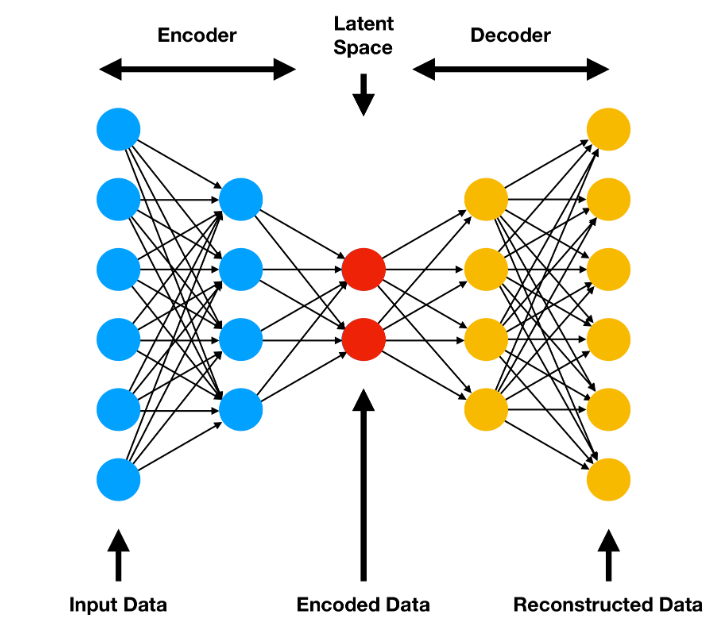
\includegraphics[width=\twoImgWidth]{images/autoencoder}%
    }%
    \hfill%
    \subfloat[\label{fig:sparseMatrix}]{%
      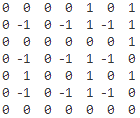
\includegraphics[width=\twoImgWidth]{images/sparse_matrix_game}%
    }%
    \captionadjust%
    \caption{\label{fig:autoencoderSparseMatrix}
    \protect\subref*{fig:autoencoder}: Example of an autoencoder network \cite{Img:autoencoder}.
    \protect\subref*{fig:sparseMatrix}: The 7x7 game state is getting more and more sparse over time.
    }%
\end{figure}

In our past work on Bomberman, we recognized the critical importance of state representation in optimizing the performance 
of our AI agents. Specifically, we focused on the transition from the original 17x17 grid, which encompassed the entire Bomberman field, 
to a reduced 7x7 grid. To accomplish this, we centered the agent's viewpoint in the 17x17 grid to capture the immediate surroundings. 
This reduction was not just a matter of simplification, it is especially important to prevent overfitting~\cite{Art:Overfitting}. When the agent network consistently 
receives the entire 17x17 field for learning, there's a high likelihood that the network will memorize training patterns and struggle with test data. 
The objective is to ensure that the agent learns the intelligent strategies of the rule-based agent to a certain extent, at the very least, mastering how 
to play the game effectively without necessarily striving for extreme efficiency. In doing so, we also took inspiration from humans who, like our AI, do not perceive 
the entire field but rather focus on a specific part while filtering out the rest.
Reducing the field to 7x7 retained key spatial relationships 
and relevant game features while simplifying the representation, thus allowing our AI agents to focus on essential information.
To determine if there is a difference in how the rule-based agent plays the game when the view box is reduced to 7x7, we had the following idea:
lets consider the following function: 
\begin{equation} \label{eq:1}
G_A(f,v) \rightarrow \{\text{up, down, left, right, bomb}\}
\end{equation}

that outputs the best possible action the agent could do. The field is described by $f$ and $v$ is the viewbox of the agent. We did many 
test rounds with the rulbased agent on an 17x17 field with \verb|--seed 1| for a comparable result. We had two scenarios
in one scenario the rulbased agent saw the whole 17x17 field e.g $G_a(f, 17\times17)$, on the other scenario the agent saw a
7x7 field e.g $G_a(f, 7\times7)$. Then we calculated the probability $p$ to find out how likely it is, that the actions in both scenarios are different in one step.
We simply counted the number of different actions and divided them by the maximum number of steps.
For the 7x7 field we had a probability of $p=0.054$ which was the best value for us compared to a 5x5 or 3x3 viewbox.\\

But, please note that initially, we interpreted this number $p$ quite differently. The probability distribution is not uniform. 
It turns out that the agent with a 7x7 viewbox makes more diverse actions as the game progresses compared to the agent with a 17x17 viewbox. 
This happens because towards the end of the game, there are fewer items or opponents within the 7x7 view, and the agent becomes uncertain about its actions. 
A better approach would be to determine the probability distribution function $p(X = k)$, where $k$ represents the number of steps in a game.
For example lets look at the probability at the beginning of the game $p(0 \geq X \leq 20) = 0$ and at the end of the game $p(310 \geq X \leq 330) = 0.47$
We had to come up with a solution to address this issue. Once the 7x7 field was empty of items or opponents, the agent switched to an exploration mode and randomly 
searched the surroundings for potential objectives.\\

However, the 7x7 field often contained sparse feature data see \autoref{fig:sparseMatrix}, with many cells remaining empty or irrelevant. 
To efficiently handle this challenge, we employed an encoder-decoder network see \autoref{fig:autoencoder}. This architecture allowed us 
to compress the sparse feature data effectively~\cite{Onl:autoencoder}. But before we delve into how the encoder-decoder network functions, we need to address how our 
features are generated within the \verb|state_to_features| function. First, we restrict the agent's field of view to 7x7. Then, we create a 7x7 map 
with the agent in the center, represented by the number 100. Here, 0 denotes open space, 1 represents crates, -1 signifies walls, 5 indicates coins, 15 represents 
opponents, and 25 stands for bombs. Another 7x7 map contains the hidden features, which are features that would otherwise overlap with those on the first map. 
These hidden features include whether all agents can ignite a bomb, represented as 0 or 1. A third map with hidden features describes the blast radius of a 
bomb along with its respective countdown. These three 7x7 maps, also known as channels, are then merged into a 
single 147-element array. Below is a code snippet:

\begin{lstlisting}[language=Python]
    ...

    def state_to_features(game_state: dict) -> np.array:
        field = game_state["field"]
        bombs = game_state["bombs"]
        explosion_map = game_state["explosion_map"]
        coins = game_state["coins"]
        agent = game_state["self"]
        others = game_state["others"]

        my_pos = make_field(agent[3])

        ...

        # non hidden features
        # make_field create a matrix from coordinate list
        channel1 = make_field(bombs) + make_field(others) + make_field(coins) 
                                     + field + my_pos

        # can agent put a bomb
        channel2 = extract_bom_is_possible_to_field(others) +  
                   extract_bom_is_possible_to_field(agent)

        channel3 = make_real_explosion_map(bombs, explosion_map)

        ...

        vf = make_viewbox(7,7, [channel1, channel2, channel3])
        return vf.flatten()

    ...
    
\end{lstlisting}

Next, we want to modify the \verb|state_to_features| function to further compress the data in the 149-element array while preserving as much information as possible. 
To achieve this, we'll utilize an encoder-decoder network see \autoref{fig:autoencoder}. This network has the same output dimension as the 
input dimension and aims to reconstruct the 
input data. However, in the dense layers, the features are reduced up to a certain point (encoded data layer). Then, in subsequent dense layers, the 
features are expanded back to the input dimension. If the network can effectively reconstruct the input data, we'll use it and extract the encoded data layer, 
which we will return in the \verb|state_to_features| function. We were able to compress the data from the 149-element array to a 72-element array. These data will 
now be used for our second network to train the rule-based agent. Details about both networks will be explained later 
in Model Architecture. Here's the modification of the \verb|state_to_features| function once again:

\begin{lstlisting}[language=Python]
    ...

    def state_to_features(game_state: dict) -> np.array:

        ...

        vf = make_viewbox(7,7, [channel1, channel2, channel3])
        compressed_features = encoder_decoder_network.encode(vf.flatten(), 72)
        return compressed_features

    ...

\end{lstlisting}

The encoder module was instrumental in feature learning, condensing the sparse data to capture essential features efficiently. 
Additionally, it reduced dimensionality, enhancing computational efficiency and reducing noise in the data. During decoding, the network could 
reconstruct the original 7x7 state representation from the compressed data, ensuring that no critical information was lost in the process.

\subsubsection*{Model Architecture}

\begin{figure}[H]
    \centering
    
    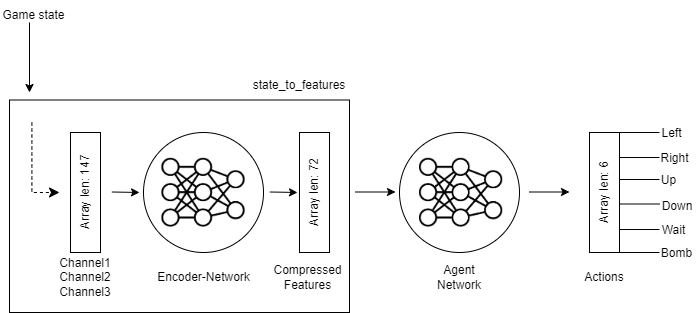
\includegraphics[width=\oneImgWidth]{images/network-arch}%
    
    \captionadjust%
    \caption{\label{fig:network-arch} Here is how our two models come into play.
    }%
\end{figure}

In total, we employ two neural networks see \autoref{fig:network-arch}. The encoder network is utilized within the \verb|state_to_features| function to compress the 
generated features, as they contain many repetitive entries, such as 0, 1, or -1. Through this compression, our aim is not only to reduce 
the data size but also to create patterns that make it easier to describe a state~\cite{Onl:autoencoder}. This is particularly significant for the second network. 
The second network is the agent network, which receives data from the \verb|state_to_features| function and endeavors to predict the best action.
Here are the characteristics of the two networks listed:

\begin{verbatim}
Encoder Network:
    Layers: 1 Inupt, 5 Hidden, 1 Output
    Neurons: 
        Input1: 147, Hidden1: 124, Hidden2: 102, Hidden3: 72,
        Hidden4: 102, Hidden5: 124, Output1: 147

Agent Network:
    Layers: 1 Inupt, 3 Hidden, 1 Output
        Neurons: 
            Input1: 72, Hidden1: 64, Hidden2: 32, Hidden3: 16, Output1: 6
\end{verbatim}

\subsubsection*{Loss function and optimizer}

We have two models: the encoder network for further feature compression and the agent network, which is tasked with 
learning how to play the game effectively. Additionally, the agent is initially meant to imitate the rule-based agent, which is 
achieved through classification. Later on, the agent will be further improved using deep Q-learning. For all these scenarios, we require 
different loss functions and optimizers with varying learning rates because there are more suitable optimizers and loss functions for specific cases.\\

For the encoder network, the ADAM optimizer with a learning rate of $0.001$ proved to be the most effective, and the chosen loss 
function was the MSE (Mean Squared Error) loss. During experimentation, we observed that the loss function did not converge to near 
zero with a learning rate of $>0.001$, and with a learning rate of $<0.001$, it converged towards zero, albeit very slowly. \\

For the agent network when mimic the rulbased agent, we used the ADAM optimizer with a learning rate of $0.0001$ and the Cross-Entropy loss function because
in classification, the goal is to assign probabilities to each class. Cross-entropy loss directly deals with probability 
distributions and can handle multi-class problems efficiently~\cite{Onl:crossentr}.\\

For the agent network during deep Q-learning, we used the ADAM optimizer with a learning rate of $0.0001$ and the Huber loss as the loss function.
It is designed to balance the benefits of mean squared error (MSE) and mean absolute error (MAE) loss functions.
But for any reason was the MSE loss better for the encoder network than the Huber loss.

\subsection{Other aproaches that we had}

At the beginning of the project, we had several other ideas about how to construct our AI agent. One alternative idea was to use Q-tables. 
For the coin collector agent, we considered the concept that it would only perceive one coin, specifically the one closest to it.
However, in the end, we discarded all of these ideas, and the following reasons explain why:

\subsubsection{Q-Tables}

Q-tables (Quality or Q-value tables) are used to approximate and store the expected cumulative rewards (Q-values) associated 
with different state-action pairs in a Markov Decision Process (MDP).
Rows represent states or state descriptions, columns represent possible actions that can be taken in those states.
Each cell in the table stores the expected cumulative reward, denoted as Q-value, for taking a specific action in a specific state.

The Q-value for a state-action pair $(s, a)$ represents the expected sum of rewards an agent can achieve by taking 
action $a$ in state $s$ and following a specific policy thereafter. The Q-value is typically updated iteratively as the 
agent explores and learns from its interactions with the environment.
Once the Q-table has converged or reached a sufficiently accurate representation of the optimal Q-values, 
the agent can select actions that maximize these Q-values

The equation for updating the Q-table in the context of Q-learning is as follows:
\begin{equation} \label{eq:1}
Q(s, a) = (1 - \alpha) \cdot Q(s, a) + \alpha \cdot [R(s, a) + \gamma \cdot \max_a Q(s', a)]
\end{equation}

In this equation:

\begin{itemize}

\item $Q(s, a)$ represents the Q-value for a specific state-action pair (s, a).
\item $\alpha$ (alpha) is the learning rate, determining the weight given to the new information when updating the Q-value. It's a value between 0 and 1.
\item $R(s, a)$ is the immediate reward received after taking action 'a' in state 's'.
\item $\gamma$ (gamma) is the discount factor, which controls the importance of future rewards. It's also a value between 0 and 1.
\item $Q(s', a)$ represents the Q-value of the next state 's' after taking action 'a', and \(a\) is the action that maximizes this Q-value.

\end{itemize}

The rason why we discarded this idea is that the bomberman environment has a large number of states, even when using a reduced state representation. 
Each cell on the game board can have multiple attributes (e.g., walls, crates, coins, enemies, bombs), resulting in an extensive state space. 
Creating a Q-table to store Q-values for every state-action pair in such a high-dimensional space would be impractical~\cite{Onl:qtabledis}.


\subsubsection{Coin-Collector Agent that sees only one coin}

Our coin collector agent was given the entire 17x17 field but only focused on the nearest coin, which was simply added to the \verb|game_state["field"]|. 
It received rewards only when collecting this specific coin. This approach worked very well for us, and the agent could consistently collect nearly 
all the coins later in the game. The advantage of this method is that it doesn't matter how many coins are on the field; the agent doesn't need to be 
retrained. However, for an agent tasked with more complex actions like defeating enemies, destroying crates, and collecting bombs, we couldn't 
pursue this idea. This is because we explored other concepts to enable the agent to perform various tasks effectively, and these concepts are described in this report.
	\newpage
	\section{Training}
	
	\fancyhead[R]{Leonie Boland}

Now that we have explored the methods that we used in our quest to train an agent to play Bomberman we are coming to the details of the training. In this section we provide a description of the training process and all strategies employed to get a good and fast result.

\subsection{Deep Q-Learning Agent} \label{sec:deepqtraining}

The following sections give an overview of the tricks utilized to train our Deep Q-learning agent. Most strategies discussed here significantly speed up the training process until a well playing agent is reached and play a very important role in our agent's implementation.

\subsubsection{Training Environment Progression}

We always conducted a similar training routine, namely starting off with a small field with height and width of 7 containing coins on every tile, so 21 coins in total. This game environment is called coin heaven in the following. Starting the training with this scenario gave us the opportunity to already evaluate if there are flaws in the implementation or how fast the network converges with the chosen hyperparameters. This is evaluated in more detail in section \ref{sec:deepqexperiments}. Then we scaled the field up to 11 $\times$ 11 and increased the difficulty by including crates. In this environment, called loot crate, we included 20 coins and used a crate density of 40\%. Finally the agent was trained with all settings as in the target field, that is a 17 $\times$ 17 field, 9 coins and a crate density of 75\%. The last step was to add opponents to this classic environment to train in the exact same environment our agent will be tested in. Simultaneously to raising size and difficulties we also increased the steps per round from 60 to 120 to 200, as the agent does not need 200 steps to collect all coins in a field as small as 7 $\times$ 7.

\subsubsection{Self-Play Strategy}

After the agent was trained without opponents to learn the basic skills like dropping a bomb to destroy crates, escaping that bomb and collecting coins, the agent needed to find out how to compete against opponents. This is where self-play comes into action. Utilizing the self-play strategy means that the model is trained while competing against itself. The advantage of this training strategy is, that the opponent has a similar level. This is desirable as a too weak opponent would not force the model to find a way to play a game more efficiently. Actually, the worst case scenario would be, that the agent learns nothing new in comparison to running the game without opponents. However, a too strong opponent would take the opportunity to learn something away from our agent, as the other opponent would collect the coins faster or kill our agent easily. Hence, we trained our agent against itself and our not training agent reloaded the model that is currently trained after every 500 rounds. As the agent improves over time, it faces progressively more challenging opponents, leading to continuous improvement and skill development. \cite{selfplay} Sadly, we only explored this strategy after handing in our best running agent at the time of the deadline. We have no data to proof that the self-play trained agent excels the previous agent but our hypothesis is, that it does.

\subsubsection{Auxiliary Rewards} \label{sec:rewards}

The basic concept of reinforcement learning is, to give the agent rewards depending on the action taken in a game state that leads to a new game state, so that the agent can learn from the rewards what to do next time it encounters a certain state. In the case of Bomberman the agent could learn the essentials to play the game by getting a reward respectively a penalty for the standard events that can occur. The standard events we chose to reward are "coin collected", "invalid action", "crate destroyed", "got killed",  "killed opponent", "killed self", "survived round" and "waited". In theory the model should be able to learn how to play the game well just by receiving appropriate positive rewards for collecting a coin, destroying crates, killing opponent and surviving one game round, and negative rewards for taking an invalid action, getting killed by an opponent or oneself and waiting. But as these rewards are very sparse the model would take a lot of time to convert the rewards into efficient moves of the agent depending on the game state. Hence to speed up the training process of the Deep-Q learning model we added auxiliary rewards that complement the standard rewards.
\\ \\
\textbf{Reward for moving towards the closest coin:} \\

\noindent First of all, we not only give a reward if the agent collects a coin but also when the agent moves in a way that brings itself closer to the closest coin. We have implemented that by looping over all coins and calculating the distance of the agent to the coins in the old game state to save the position of the closest coin. Then we compare the distance of the agent to that closest coin in the old versus the new game state. If the distance got smaller the reward is 10 divided by the old distance. This way getting closer to a coin is more important when the coin is close in comparison to when the coin is far away. We chose that gradation of the reward because an opponent could get to the coin faster anyway when it is too far away from our agent, or there might be a better action to do, like dropping a bomb to destroy many crates, instead of moving toward that far away closest coin. If the agent has the same distance to the closest coin in the old and new game state it is rewarded with 0.5. 

The third option is, that the agent moves away from the closest coin, but in this case we have to take a closer look, as it might be necessary to move away from the coin to actually get to the coin at all in the end. Hence, we check if the direct way to the coin is blocked by a wall, in which case the agent would need to move a tile in a direction that brings it further away from the coin. This scenario is showcased in Figure \ref{fig:coin-blocked}. This would be rewarded the same way as keeping the same distance to the coin, so with 0.5. Otherwise, if the agent moves away without the need to, it gets a negative reward of 10 divided by the new distance to the closest coin, with the same justification as explained before.

\begin{figure}[H]
	\centering
	
\includegraphics{images/coin_blocked.png}
	\caption{In this extract of Bomberman the agent is positioned only two tiles away from the closest coin, but a wall is blocking the direct way to the coin. So by moving up or down one tile the agent would be three tiles away from that coin. However, this step is necessary to get to the coin at all, so here it is not penalised to move away from the coin, like it normally is.}
	\label{fig:coin-blocked}
\end{figure}

\noindent \textbf{Rewarding each crate that will be destroyed by a dropped bomb and considering the necessity of a dropped bomb:} \\

\noindent Next we included two reward functions that are closely related to each other, namely a function counting and rewarding all crates that will be destroyed by a bomb dropped by our agent and another function penalising or rewarding the necessity of a bomb dropped by our agent. To count all crates that are lying in the bomb's explosion radius we have to check each tile that is impacted by the bomb for the existence of a crate. To do that we need to be sure that the index of the potential explosion radius is part of the game's field and if there is a crate it could be protected by a wall blocking the explosion. Every crate that will be destroyed by a bomb gives an extra 5 point reward. If no crate will be destroyed the reward is -5. 

Additionally, the bomb necessity reward function monitors if there is a opponent in a 7 $\times$ 7 field around the dropped bomb because this opponent could potentially move into the explosion radius. Every opponent fulfilling this condition brings an extra 2 point reward, while the action of dropping a bomb in a position where no opponent is in the 7 $\times$ 7 field and no crate will be destroyed results in a negative reward of 22.
\\ \\
\textbf{Punishment for a dropped bomb without an escape route:} \\

\noindent In regards to bombs dropped by our agent we introduced one more reward, as one of the worst moves an agent can do in this game is dropping a bomb that the agent cannot escape from. Consequently, we penalised this very hard with -100.

To control if there is an escape route we initialized four variables, each variable illustrating one direction in which the agent could escape, with False. Then the implementation works its way from the outside to the inside, first looking if the tiles outside of the bomb's explosion radius in all four directions are free, which turns the boolean variable accordingly to True. Next, one tile closer to the bomb, we check if this tile is free and one of the adjacent tiles, that are not affected by the explosion, are free too. This would result in changing the corresponding direction variable to True as the agent would be able to escape to these adjacent tiles in time before the bomb goes off. However, if the tile on the way to the adjacent safety spots is blocked by a wall or crate the variable is changed back to False even when it could have been True before. This is done again for a tile even closer to the bomb, and so on, for all four directions.

Concluding, we have four variables that state whether in a direction, so to the bottom, top, left or right, there is an escape route or not. If any of these variable's values is True there is an escape route and the agent is rewarded with 2 for dropping a bomb that it can escape from. Otherwise, as mentioned before, the punishment is -100.
\\ \\
\textbf{Assess movements made by the agent in regards to all bombs on the field:} \\

\noindent Lastly, the agent has to pay attention to every bomb, not only its own bombs and eventually move to safety. With our final reward function called bomb radius we gave the agent positive feedback when moving away from a bomb and finding a safe spot and negative feedback if the agent moves back into a bomb radius or gets closer to a bomb. To do so, we first examine if the agent is positioned on the same spot as a bomb, so probably the bomb we are dealing with is a self dropped bomb. Then we use the function explained above that determines the possible directions that the agent can escape to and reward the agent for moving in a direction where it is possible to escape. On the other hand, of course the agent is punished with a negative reward for going in a direction without a possibility to escape. 

If the agent is not positioned on the exact same x- and y-positions of a bomb but rather one coordinate, so either x- or y-coordinate, overlap with a bomb we have to take a couple of cases into consideration. First, is a wall protecting the agent from the explosion anyway? If the answer to this question is yes we are not interested in rewarding the move the agent does because it was not in danger in the first place, and cannot move into the danger zone of this bomb with one action. Without a protecting wall, the question is whether the agent is too close to a bomb, so that the explosion would kill the agent. In this case the agent gets a small reward for moving away but still being in the bomb's radius and a higher reward for moving to a tile that will not be affected by the bomb's explosion. However, if the agent does not move away it is punished. There is also the possibility that the agent was not in the bomb radius and moved into it, which gets punished as well. The same is done in the third case, that the agent had no overlapping coordinates but moved into the bombs radius.

The reward, no matter if positive or negative, determined by all the above mentioned if-cases is multiplied by 4 subtracted by the count down until the bomb explodes, which ranges from 3 to 0. So if the bomb was just dropped and has a count down number of 3, the reward stays the same as it is multiplied by 1. On the other hand, if the bomb goes off soon, so the count down number is 0 the reward is multiplied by 4. By including this multiplication we hoped to emphasize the need to get out of the way of a bomb if it detonates soon. Additionally, the agent should not hesitate to move through a bomb radius to, for example, come closer to a coin if the count down of a bomb is still high.
\\ 

All of these auxiliary rewards needed to be adjusted such that the agent understands the priorities of the game and does not make unnecessary moves due to bad rewarding. Eventually, our final agent learned how to play the game fairly efficient after a total of 100,000 rounds of training in different scenarios with different settings, which would not have been possible with only the standard rewards.

\newpage
\fancyhead[R]{Kevin Klein}
\subsection{Imitation-based RL Agent}

In this section, we describe how we trained our second-best agent. This agent initially imitates 
the rule-based agent and then seeks further improvement through Deep Q-learning.

\begin{figure}[H]
    \centering
    
    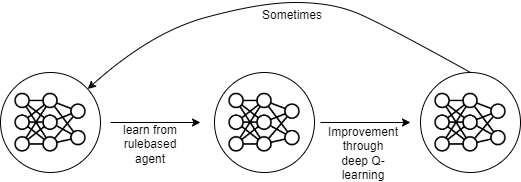
\includegraphics[width=\oneImgWidth]{images/training-strategy}%
    
    \captionadjust%
    \caption{\label{fig:training-strategy} Here is how we trained our second best model.
    }%
\end{figure}

Our initial idea was to develop an agent that starts by performing at the same level as the rule-based agent and then improves 
further through Deep Q-learning. For this purpose, we had devised the following concept see \autoref{fig:training-strategy}.

Initially, our agent attempted to imitate the rule-based agent, as mentioned earlier. This was achieved through a classification approach. 
We collected the actions of the rule-based agent for each game state, and these actions served as the labels for the respective states. 
We gathered between 500,000 and 1,000,000 action-label pairs in this manner.
New data was added to the ReplayBuffer after each step until reaching the limit of 500,000 to 1,000,000 entries. 
After each round, specifically at the \verb|end_of_round| event, the following simplified function was executed to train our model.
Of course, the model was then also saved in an external file, which was achieved using Pickle.

\begin{lstlisting}[language=Python]
    ...
    
    def learn_rulebased_agent(model, labels, data, loss, opt, batch_size):
        train_ds = CTDataset(data, labels)
        train_dl = DataLoader(train_ds, batch_size=batch_size, shuffle=True)
        epoch_loss = 0

        ...

        for epoch in range(NUM_EPOCH):
            print("epoch %d / %d" % (epoch + 1, NUM_EPOCH))
            for i, (x, y) in enumerate(train_dl):
                opt.zero_grad()
                pred = model(x)
                loss_value = loss(pred, y) 
                loss_value.backward() 
                opt.step()
                epoch_loss += loss_value.item() 

            if epoch_loss <= 1e-5:
                break

            print(f"loss/epoch: {epoch_loss}")
            epoch_loss = 0      

    ...
    
\end{lstlisting}

First, we pass the model to the function that we want to train, followed by the labels, 
which represent the actions of the rule-based agent, and the data, which corresponds to the states. 
Then, we provide the loss function and optimizer, and finally, the batch size. We found that a batch size of 1024 worked well for us, 
especially as the model had more data to train on when the ReplayBuffer became fuller. We did experiment with other batch sizes,
but if the batch size was too small, it took a long time for the loss function to converge to 0 (which it did not entirely reach).

We achieved good results when the \verb|num_epoch| was initially set at 2000, which we later increased to 5000 during training. 
Additionally, we sometimes had to remove older data from the ReplayBuffer to ensure that the model continuously learned from new games. 
It was also worthwhile to reduce the view box to 7x7 because it significantly reduced the number of possible states. 
After 4-5 days of training, our model became reasonably proficient at playing the game. While it could not perfectly mimic the rule-based agent, 
as the agent occasionally had to make random moves when there were no more items in its 7x7 view box, we still found the results quite satisfactory.

Afterward, we attempted to enhance the model using Q-learning. For this, we utilized the reward functions from our best agent in the first project. 
Unfortunately, this approach did not work well; the agent's performance deteriorated, and eventually, it struggled to play the game effectively. 
We saw improvement when we alternated training the model with the rule-based agent and then applied Deep Q-learning, see \autoref{fig:training-strategy}. 
However, even in this scenario, 
the results were significantly worse compared to when our model was solely imitating the rule-based agent.

In the end, we were unable to improve the agent using Q-learning beyond the level of our initial project, 
which we naturally submitted. We also considered reasons why we could not enhance the agent pre-trained with rule-based 
data using Deep Q-learning. The main issue likely stems from optimizing the model with vastly different values when it imitates 
the rule-based agent compared to when it undergoes Deep Q-learning. In the first case, the model is optimized with one-hot encoded 
actions of the rule-based agent, while in the latter case, it is optimized with the values of the reward function and the next states.
	\newpage
	\section{Experiments and Results}

	\newpage
\fancyhead[R]{Leonie Boland}
\subsection{Deep Q-Learning Agent}

In this section we are giving an overview of the experiments we have done with our deep q-learning model that lead to our best performing agent. The basic framework is already described in the sections Methods and Training (give reference here). Hence at this point we trained the model, evaluated the performance and based upon that we changed hyperparameters or auxiliary rewards to improve the model.\\ \\
Initially, most experiments resulted in the fine tuning of the rewards and auxiliary reward functions. A good indication that the rewards are not helping the model to get trained in the most efficient way is a big deviation between the sum of the rewards in comparison to the score achieved by the agent. Ideally the score in the end of a round is constantly high if the sum of the rewards is high too, especially if the rewards' sum is in a high range for many rounds already, so if it has converged. The plots in Figure \ref{fig:rewardVSscore} show an contrary example of this phenomenon when the model was trained for 10000 rounds in the 7 $\times$ 7 coin heaven scenario. These plots do not show one straight line but a constantly changing reward sum respectively score on a high scale x-axis. This is why the plots come off rather chaotic than organized, but they still depict the training's progress. In this example there is a quite sudden improvement in the score between the 2000th and 3000th round of training and this jump can also be observed in the rewards plot on the left but is much less significant. Furthermore, the rewards still increase and seem to have converged after the 5000th round of training. Nonetheless the score is getting worse and keeps fluctuating between the highest possible score 21 and a score as low as 3. This means, that even though the model obviously has not found a good way for the agent to run in the coin heaven environment the rewards, that it is receiving, indicate exactly that the way the agent acts is good. When letting the agent play we noticed that this happened because the agent dropped many unnecessary bombs and thus killed itself occasionally, so the agent was not able to collect all the coins. However the total amount of rewards was still high because the agent was remunerated a lot for outrunning a bomb and was not punished for dropping a totally unnecessary bomb. We understood the background of this behavior by consulting the logged messages parallel to training the agent a few rounds with the GUI (Graphical User Interface) turned on. Therefore we fine tuned the rewards with a closer examination of matching the extent of rewards for different actions with each other. We also added a penalty for dropping bombs that will not destroy crates or are in reach of an opponent as described closely in section \ref{sec:deepqtraining}. 
\begin{figure}[H]
	\centering
	\begin{minipage}{0.49\textwidth}
		\centering
		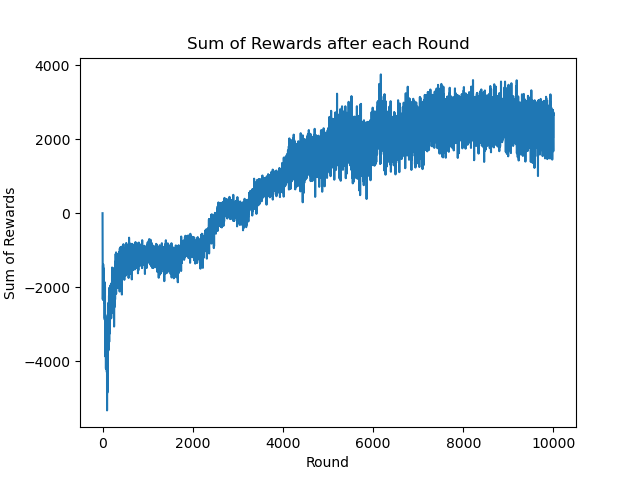
\includegraphics[scale=0.52]{images/rewards_converged.png}
	\end{minipage}
	\begin{minipage}{0.49\textwidth}
		\centering
		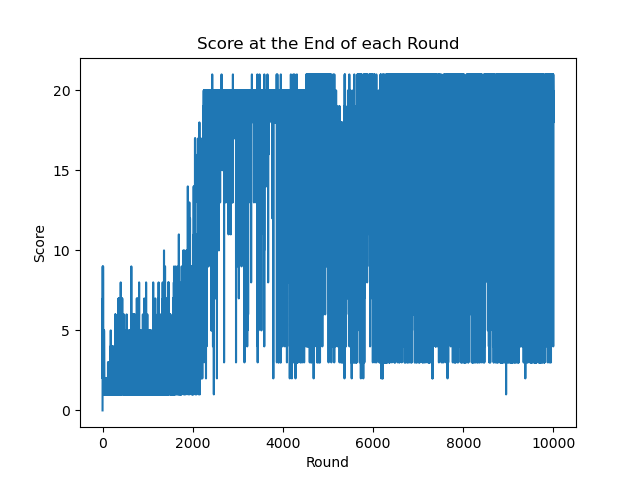
\includegraphics[scale=0.52]{images/scores_not_converged.png}
	\end{minipage}
	\caption{Both plots were generated during the training of the Deep Q-Model on a small coin-heaven scenario with coins on every free tile. The x-axis of both plots represents the rounds of the training. While the left plot depicts the sum of all rewards given to the agent in each round, the right plot shows the score after each round. These plots show discrepancy between rewards and scores.}
	\label{fig:rewardVSscore}
\end{figure}

After more test runs and improvements of the auxiliary rewards we were already able to produce a model that collected all coins efficiently. Figure \ref{fig:efficientCoinHeaven} shows the corresponding rewards and scores of 8000 rounds of training. This time score and reward coincide very well. Again, between the 2000th and 3000th round there is a steep increase of rewards and scores where the model apparently found a good way to handle this environment. Henceforward, both scores and rewards, are on a constantly high level. Of course, there is still a certain amount of fluctuation between each round as the agent is supposed to do some random moves during training to find a potentially better way of playing the game. Here the probability of doing a random move during training, not calculated by the network, was constantly 10\%.
\begin{figure}[H]
	\centering
	\begin{minipage}{0.49\textwidth}
		\centering
		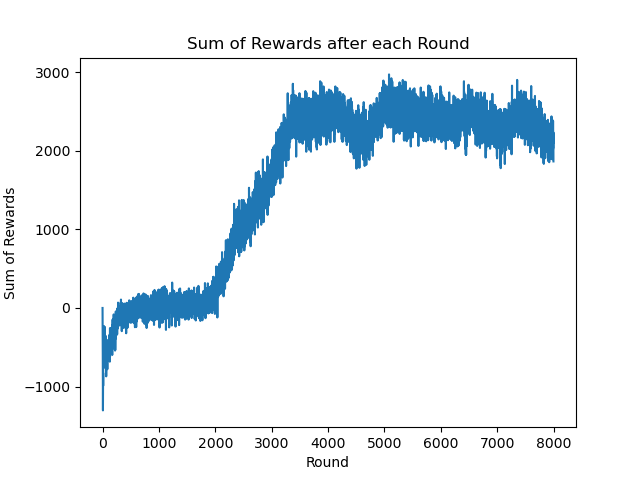
\includegraphics[scale=0.52]{images/rewards_perfect_coinheaven.png}
	\end{minipage}
	\begin{minipage}{0.49\textwidth}
		\centering
		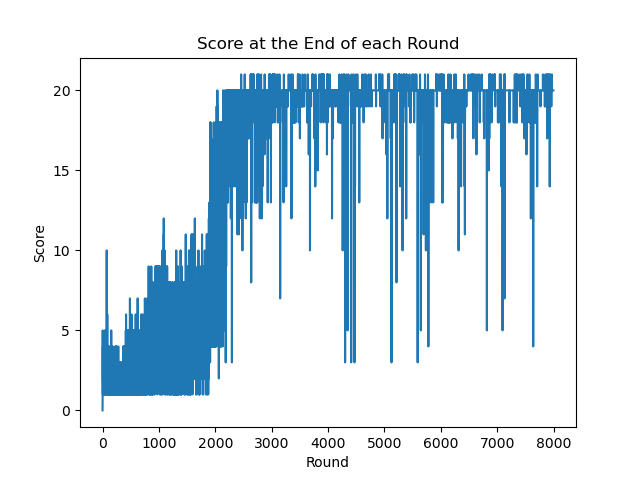
\includegraphics[scale=0.52]{images/scores_perfect_coinheaven.png}
	\end{minipage}
	\caption{The plots are constructed in the same way as described before, but after the reward fine-tuning. The scores shown here fit to the high reward sum.}
	\label{fig:efficientCoinHeaven}
\end{figure}

Although the auxiliary reward functions seemed to be elaborated very well at this point, the agent did not play smoothly on larger fields in the harder levels even after a lot of training rounds. The main concern was that the agent often kept killing itself in early steps of the game. With the assumption that the rewards are handed out reasonably we also had to evaluate other hyperparameters. Our neural network consisted of a very simple architecture so we thought about features to add to the network to enable better learning. Even though dropout is a very common property to have in neural networks, it did not make sense for our task as it is used to prevent overfitting, which cannot happen here. Instead we included batch normalization which should stabilize and accelerate the training \cite{batchnorm}. The batch normalization layers were placed before adding the four parallel models together as batch normalization after the concatenation normally leads to worse results \cite{batchnormpos}. Unfortunately when doing the training from scratch the batch normalization did not result in a better running agent or a faster training, probably because the batch size was too small. Not only was the batch size small in general with 256, but we could not collect enough training samples if the agent killed itself early in the game. This did not allow the positive effects of batch normalization to unfold in our network. Furthermore batch normalization is more efficient in deeper networks \cite{batchnorm}, but with one hidden layer our neural network is rather shallow.

Next we gave different loss functions a try. We initially used the smooth L1 loss but also thought of trying the cross-entropy loss because it is the standard loss for classification models, where the output usually is a list of probabilities. In our case the output gives the probability of an action to be the best action to take in the current state of the game for every possible action. Applying the cross-entropy loss showed that our model is not suited for this kind of loss. A reason for this could be that we want to find a good metric to calculate the loss between the predicted and the target q value, calculated following the Bellman equation. The literature hints that we should minimize the quadratic error between those values. In the formula for the cross-entropy loss presented in section \ref{sec:crossentropy} the quadratic error is not calculated. Instead, loss functions that can be considered next to the Smooth L1 loss is the closely related Huber loss and of course the MSE loss. In the end the MSE loss proofed to be most efficient, so our final agent was also trained with this loss. When discussing the loss we also inevitably gave thought to the optimizer. The AdamW optimizer worked well but RMSprop was more effective. Especially the faster convergences shown in Figure \ref{fig:adamvsrmsprop} was a decisive point in favor for the RMSprop optimizer. Thus we proceeded with RMSprop, but as AdamW achieved good results too, we believe that an agent trained with this optimizer would haven been able to run similarly when giving more consideration to the learning rate.
\begin{figure}[H]
	\centering
	\begin{minipage}{0.49\textwidth}
		\centering
		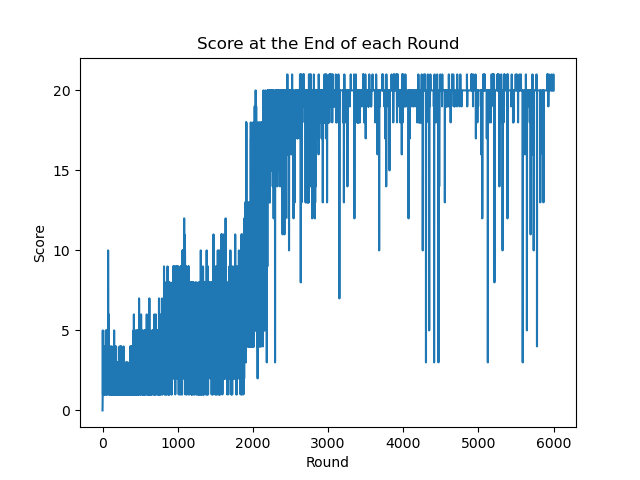
\includegraphics[scale=0.52]{images/scores_adamw.png}
	\end{minipage}
	\begin{minipage}{0.49\textwidth}
		\centering
		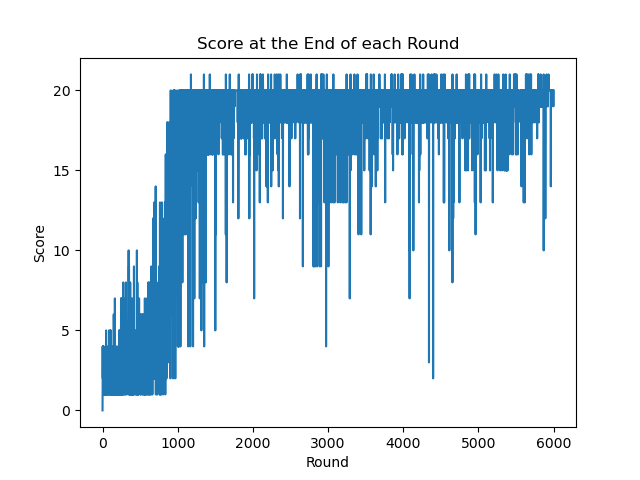
\includegraphics[scale=0.52]{images/scores_rmsprop.png}
	\end{minipage}
	\caption{The plots are constructed in the same way as before, but both plots depict the scores of to different trainings. The left one was trained with the optimizer AdamW and the right one was trained with RMSprop. The model using RMSprop improves and converges faster.}
	\label{fig:adamvsrmsprop}
\end{figure}

With the configurations chosen as explained above we reached a fairly good playing agent after 6000 rounds of training in coin heaven (7 $\times$ 7 field, coins on every free tile and 60 steps per round), 60000 rounds of training in loot crate (11 $\times$ 11 field, 20 coins, 0.4 crate density, 120 steps per round), 15000 rounds of training in classic (17 $\times$ 17 field, 9 coins, 0.75 crate density, 200 steps per round) and 40000 rounds of training in the classic scenario as described before but with two rule based agents and one coin collector agent as opponent. Strangely, except of being able to play the game well the agent did not learn to not do invalid actions. We observed that the majority of self killing happened because the agent still did invalid action, like trying to move in a direction, where a wall is located, to escape a bomb. Thus, to get a better playing agent we force the agent to not do invalid actions in the not-training mode. After each neural network output we check if the chosen action, so the action with the highest probability, can be executed and if not we take the action with the second highest probability and check this one. This is done until a valid action is found. 

Finally, we created an agent that can compete with a rule based and coin collector agent but is mostly not able to beat them. Still, we can conclude that our model did learn how to play the game as it clearly outperforms a random agent, which nearly always makes 0 points. Figure \ref{fig:game1} shows the scores of four agents, namely our reinforcement learning agent, a rule based agent, a coin collector agent and a random agent, when they play against each other in the classic scenario for 10 rounds. We also found that our agent performs better against stronger agents, maybe because it was trained against strong agents. When we choose the same opponents as during training, so 2 rule based agents and 1 coin collector, our agent often outperforms at least one of them.
\begin{figure}[H]
	\centering
	\begin{minipage}{0.49\textwidth}
		\centering
		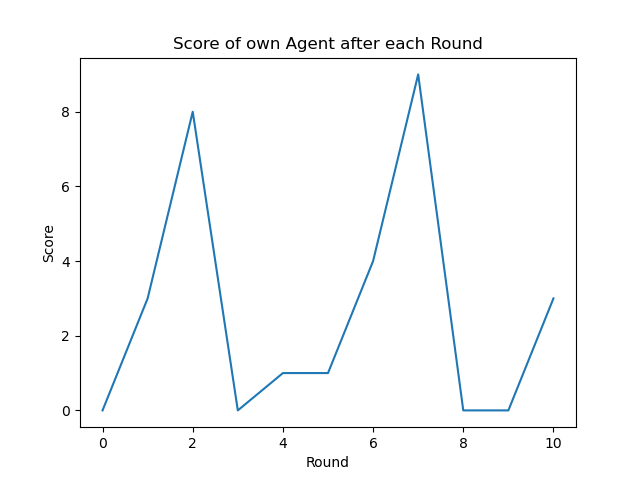
\includegraphics[scale=0.52]{images/my_scores11_1.png}
	\end{minipage}
	\begin{minipage}{0.49\textwidth}
		\centering
		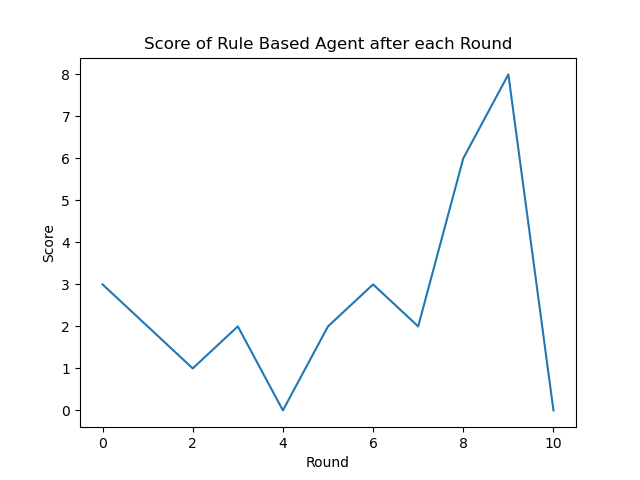
\includegraphics[scale=0.52]{images/rule_scores11_1.png}
	\end{minipage}
	\begin{minipage}{0.49\textwidth}
		\centering
		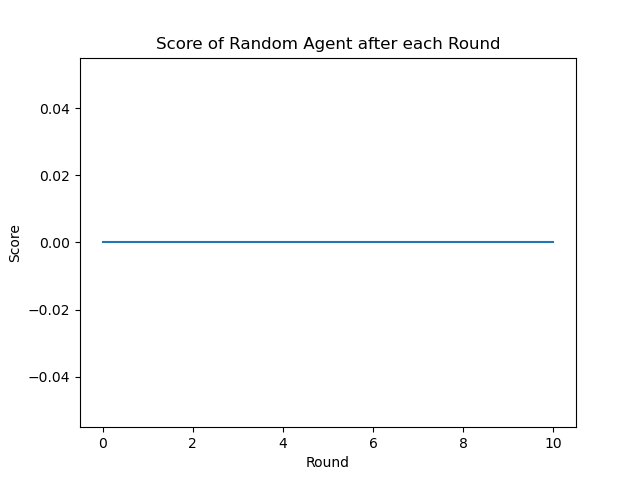
\includegraphics[scale=0.52]{images/random_scores11_1.png}
	\end{minipage}
	\begin{minipage}{0.49\textwidth}
		\centering
		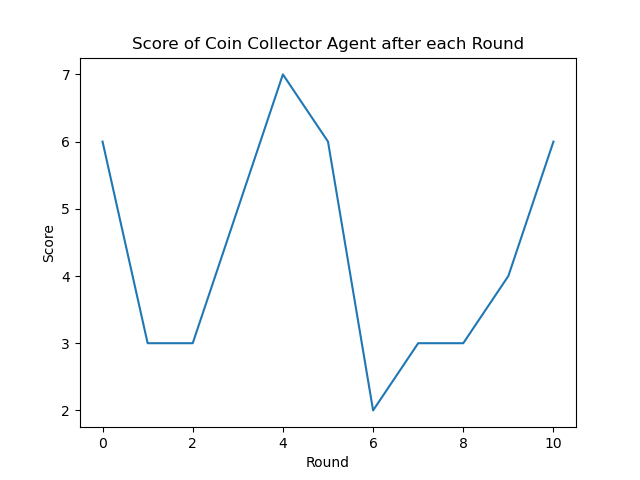
\includegraphics[scale=0.52]{images/coin_scores11_1.png}
	\end{minipage}
	\caption{These plots result from one game of bomberman with 10 rounds. Our reinforcement learning agent represented in the top left, played against a rule based agent represented in the top right, a coin collector agent represented in the bottom right and a random agent represented in the bottom left. While the random agent did not score any points, our agent and the rule based agent both scored 29 points in total and the coin collector won with 46 points.}
	\label{fig:game1}
\end{figure}

Currently our agent still has a few problems when playing the game. It kills itself sometimes by not escaping or escaping in a direction where the agent cannot get to safety. In consideration of our auxiliary rewards explained in section \ref{sec:rewards} this is a phenomenon that we did not expect as the auxiliary rewards are designed exactly to avoid this. Thus we hoped that the agent would learn quite early how to escape its own bombs. So unfortunately, due to time restrictions, we could not test whether more training solves the problem but we assume that it would not. This leaves us with the believe that there are still flaws in our model, the state to feature function or the auxiliary rewards. (VIELLEICHT EHER IN CONCLUSION?). Another undesired behavior is that the agent sometimes just stops moving even though there are still crates to destroy and coins to collect. Instead of stop moving it also sometimes gets caught in a loop, like just moving up and down all the time. All the same, the agent still escapes a bomb that is dropped by an opponent when it is too close. Sometimes we also observe that this can trigger the agent to move efficiently again. One reason for that could be that in our state to feature function we gave the agent only a 7 $\times$ 7 vision field with all the details it needs about crates, coins, opponents and bombs. We expected this to be a problem from the beginning so we included our so called outside map collecting information happening outside of this vision field, so that the agent still knows what is going on farther away. Probably this still is not enough to keep the agent moving especially as it is only directly rewarded for any movement if it is getting closer to a coin. Nonetheless it should be worthwhile for the agent to move towards crates and destroy them in the long run. Maybe this is a behavior that could be improved by more training even though the reward plots seem to show some convergence we never know if there could happen another positive adjustment to the agent after more training rounds.

	\newpage
\fancyhead[R]{Kevin Klein}

\subsection{Our second best agent}

In this section, we present the results of our second-best agent, which was intended to learn to mimic the rule-based agent initially and 
then be improved through deep Q-learning (which, as it turned out, did not work well). We illustrate the training process to imitate the rule-based 
agent and the subsequent training with deep Q-learning using diagrams.

\begin{figure}[H]
    \centering
    
    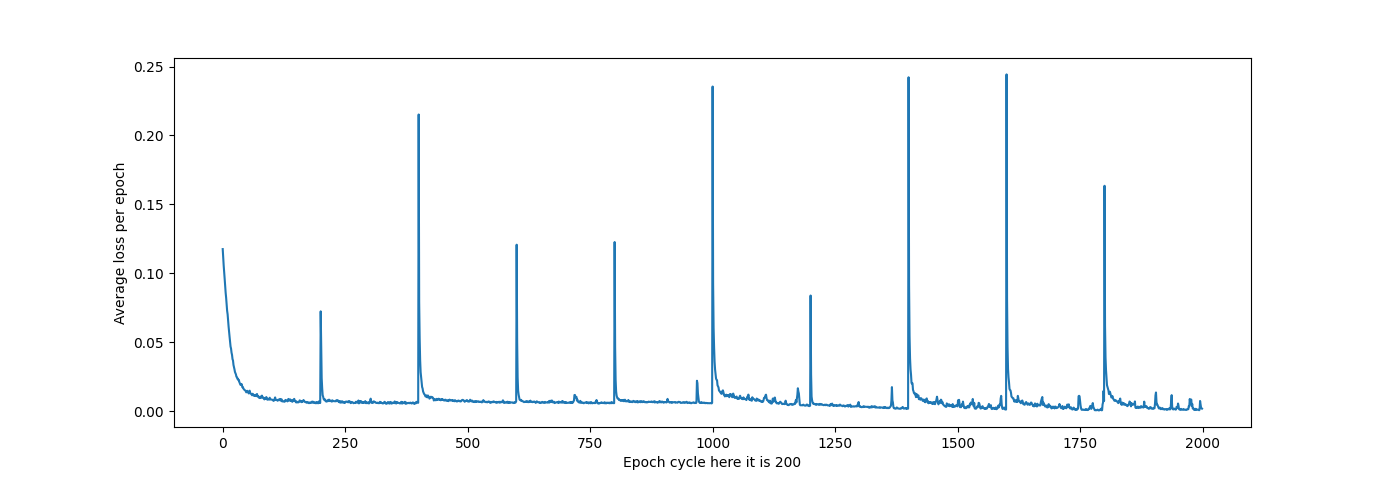
\includegraphics[width=\oneImgWidth]{images/secondAgentTrainChart1}%
    
    \captionadjust%
    \caption{\label{fig:secondAgentTrainChart1} Here is  the training progress for imitating the rulbased agent at the beginning of our second best model.
    }%
\end{figure}

At the beginning of training, our agent aims to imitate the rule-based agent. For this purpose, the ReplayBuffer was filled with data 
from the rule-based agent. After each round, the agent was trained with the current data from the ReplayBuffer. At the start of the training, 
the buffer was relatively empty and had few data points. It took some time to reach a capacity of 500,000. In \autoref{fig:secondAgentTrainChart1}, you can observe 
this (we set \verb|NUM_EPOCH| to 200 here for better visualization). Each time 200 epochs were completed, a new training round began, and the 
ReplayBuffer collected new data. Since the buffer had few data points, new data made up a significant portion, leading to noticeable spikes 
in the loss function at the beginning of each 200-epoch cycle, as seen in \autoref{fig:secondAgentTrainChart1}. This behavior will improve over the course of training, not 
only because the buffer will have more data but also because the agent will learn from it.

In the end, our goal was to eliminate these spikes completely. This indicates that the agent can handle new game states effectively. 
To achieve this, we increased the number of epochs during training and removed old data from the ReplayBuffer. Additionally, we dynamically 
adjusted the batch size. When the buffer had few data points, the batch size was 32, later increased to 512, and eventually set to 1024.
By the way, the training process for the encoder network followed a similar pattern; we simply reduced the dataset size to 100,000. Otherwise, 
the graph looked almost the same, except that the level of the loss function was higher, so it never reached 0.

\begin{figure}[H]
    \centering
    
    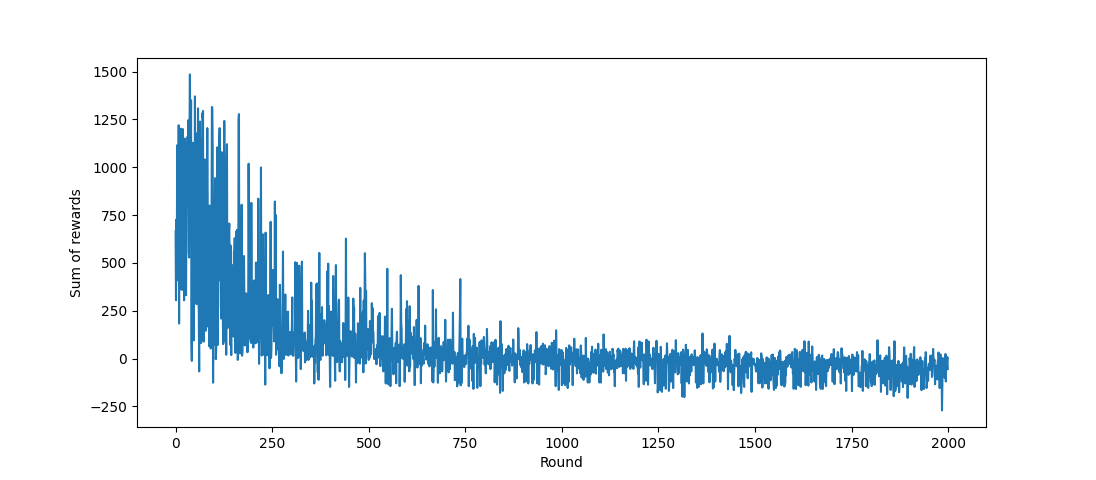
\includegraphics[width=\oneImgWidth]{images/secondAgentTrainChart2}%
    
    \captionadjust%
    \caption{\label{fig:secondAgentTrainChart2} Here is the training progress as we attempted to enhance the agent performance using deep Q-learning.
    }%
\end{figure}

After the agent achieved a decent level of play through training with the rule-based agent, our goal was, of course, 
to further enhance its performance to enable it to defeat other rule-based agents in the game. We thought the agent could 
leverage the knowledge of the rule-based agent and then learn better or different strategies more easily and quickly. 
However, as observed in \autoref{fig:secondAgentTrainChart2}, that was not the case. With increasing training, the agent's performance deteriorated, 
reaching a point where it could no longer play the game. Even when we increased the number of rounds to 20000, there was no improvement. 
We tried various approaches, such as changing the loss function, optimizer, learning rate, and so on, but nothing helped. We suspected that 
one possible reason for this issue was the use of different training sets with labels that were entirely 
differently dimensioned, which might have caused the problem.
	\newpage
	\section{Conclusion}

 	\fancyhead[R]{Leonie Boland}

\subsection{Deep Q-Learning Agent}

In summary, the approach of using Deep Q-Learning to play Bomberman with reinforcement learning was successful. Once the main framework was in place, we found that it is very important to give a lot of thought into the rewarding and auxiliary rewards as the performance of the agent depends crucially upon that. Certainly, fine tuning hyperparameters also plays an important role, but as soon as the model was running well, there seemed to be no big differences in the performance based on hyperparameter changes.

The model does not provide a perfect performance as explored in the end of section \ref{sec:deepqexperiments}. With the given time constraints we are only able to give hypotheses for the reasons of the malfunctions. Our believe is that, most of the deficits might resolve when working out a better way to implement the state to feature function or the auxiliary rewards.

 	\newpage
	\fancyhead[R]{Kevin Klein}
\subsection{Imitation-based RL Agent}

In conclusion, our attempt to develop an agent that initially imitated the rule-based agent and then enhance its capabilities using Q-learning led 
to mixed results. The training to imitate the rule-based agent was more or less successful, and the agent demonstrated promising performance, aligning with the rule-based 
strategies in a certain point. However, when we introduced Q-learning to further improve its gameplay, the results were disappointing. Instead of enhancing its skills, 
the agent's performance steadily declined during training, reaching a point where it was unable to play the game proficiently.

We hypothesized that a significant factor contributing to this issue was the disparity in the dimensionality of the training sets 
used for imitation and Q-learning. The transition from the well-structured imitation training data to the Q-learning dataset, which likely 
had different dimensions and characteristics, might have caused confusion and hindered the agent's learning process. This mismatch in the training sets 
could have led to the deterioration in performance, highlighting the importance of consistent and compatible data when implementing reinforcement learning techniques. 
Further investigations and refinements in the training process are necessary to address these challenges and achieve successful integration of imitation learning and
Q-learning for optimal agent performance in the game.

\subsubsection{Outlook}

The biggest problem with our approach was that the agent kept getting worse during Deep Q-Learning, 
even though it performed quite well through training with the rule-based agent. However, we do not want 
to abandon this approach in the future. It needs to be analyzed what the reasons for this were.
It might be beneficial to mix the two training approaches instead of keeping them separate.

	\newpage	
	\pagestyle{plain}
	%\nocite{*}
	\printbibliography
\end{document}
